\chapter{Sprint 3}
	
\section*{Introduction}
    The third sprint of the project's life cycle started on a team-wide planning meeting and resulted in the following:
    \begin{itemize}
        \item This sprint is spread out over five weeks
        \item  At the end of this sprint, the Travel order module will be delivered as well as the first release of the project. 
        \item Development of the sprint 3 Backlog
        \item Elaboration of a design phase
    \end{itemize}
\subsection*{Purpose of the module}
This module is the main module of our project, In this module, the travel order is created, processed, and closed. Each of the actors has his role in this module but it all boils down to basic workflow.
\subsection*{Actors}
\begin{itemize}
\item \textbf{User}: Creates and manages his travel orders.
\item \textbf{Manager}: Confirms draft and validates agents' work.
\item \textbf{Agent}: Process the travel orders
\end{itemize}
\subsection*{Travel order phases}
The figure below shows all the order states in the workflow.
\begin{figure}[H]
    \begin{center}
        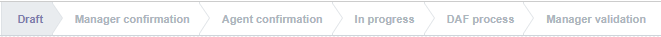
\includegraphics[scale=0.9]{img/workflow.png}
        \caption{travel order workflow}
    \end{center}
        \label{fig:my_label}
\end{figure} 
And in this flowchart diagram we go over them:
    \begin{center}
        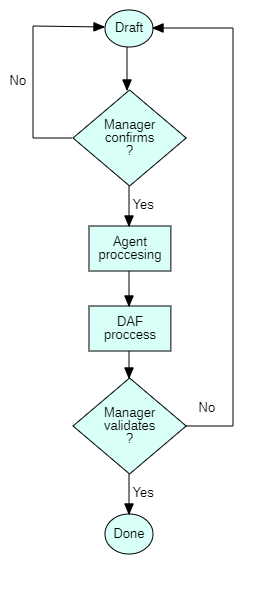
\includegraphics[scale=0.6]{img/workflow2.png}
        \caption{travel order flowchart diagram}
    \end{center}
\section{Sprint backlog}
The following table summarizes the tasks that we are responsible for carrying out 
\begin{center}
\begin{longtable}{|p{1cm}|p{6,25cm}|p{0,7cm}|p{6,25cm}|p{0,8cm}|}
\caption{ Project backlog }
\hline
\textbf{US ID} 
&\textbf{User Story}
&\textbf{T ID}
&\textbf{Task}
&\textbf{Esti- ma- tion}
\\
\hline
\multirow{ 3}{*}{0}
&\multirow{3}{*}{Storyless}
&0.1
&Class diagram
&4h\\\cline{3-5}
&
&0.2
&Use case diagram
&8h\\\cline{3-5}
&
&0.3
&Documenting progress
&2h\\\cline{3-5}
\hline

\multirow{2}{*}{19}
&\multirow{2}{=}{As a User , I want to be able to create, edit and delete travel order drafts}
&19.1
&Create the «Mission» model
&8h\\\cline{3-5}
&
&19.2
&Create the «Mission\_form» view
&2h\\\cline{3-5}
&
&19.3
&Create the security rules
&30m\\\cline{3-5}

\hline


\multirow{ 2}{*}{20}
&\multirow{2}{=}{As a User , I want to be able to see all my travel orders}
&20.1
&Create the «ETM Mission» menu
&30m\\\cline{3-5}
&
&20.2
&Create the «My Orders» menu item
&30m\\\cline{3-5}
&
&20.3
&Create the «User\_Dashboard» view
&4h\\\cline{3-5}
\hline


\multirow{2}{*}{21}
&\multirow{2}{=}{As a User , I want to be able to filter my travel orders by status or date}
&21.1
&Add status filter to the «User\_Dashboard» view
&4h\\\cline{3-5}
&
&21.2
&Add date filter to the «User\_Dashboard» view
&4h\\\cline{3-5}

\hline

\multirow{3}{*}{22}
&\multirow{3}{=}{As a User , I want to be able to file my travel order drafts and track their progress}
&22.1
&Create the «workflow.xml» view
&8h\\\cline{3-5}
&
&22.2
&Add  «Confirm» action to the draft view
&2h\\\cline{3-5}
&
&22.3
&Add status indicator to the «User\_Dashboard» view
&2h\\\cline{3-5}

\hline

23
&As an Agent , I want to be able to see all travel orders
&23.1
&Create the «Agent\_Dashboard» view
&8h\\\cline{3-5}

\hline

\multirow{2}{*}{24}
&\multirow{2}{=}{As an Agent , I want to be able to add attachments to travel orders}
&24.1
&Create the «Add\_Attachments» widget
&6h\\\cline{3-5}
&
&24.2
&Create attachment constraints and verification
&2h\\\cline{3-5}
\hline

\multirow{2}{*}{25}
&\multirow{2}{=}{As an Agent , I want to be able to change travel orders’ status}
&25.1
&Add «Agent\_confirm» action to the workflow
&4h\\\cline{3-5}
&
&25.2
&Add «Agent\_deny» action to the workflow
&4h\\\cline{3-5}
\hline

\multirow{2}{*}{26}
&\multirow{2}{=}{As a Manager , I want to be able to see all travel orders pending my confirmation}
&26.1
&Create the «Manager\_Dashboard» view
&6h\\\cline{3-5}
&
&26.2
&Add menu item «Management» to main menu
&30m\\\cline{3-5}
\hline

\multirow{2}{*}{27}
&\multirow{2}{=}{As a Manager , I want to be able to confirm or reject travel orders pending my confirmation}
&27.1
&Add «Manager\_confirm» action to the workflow
&4h\\\cline{3-5}
&
&27.2
&Add «Manager\_deny» action to the workflow
&4h\\\cline{3-5}
\hline


\end{longtable}
\end{center}


\section{Software Design}
Like the previous iterations we elaborate a conceptual study or we use UML diagrams to have a more in-depth view on the module.
    
         \subsection{Use case diagram}
    \begin{figure}[H]
    \begin{center}
        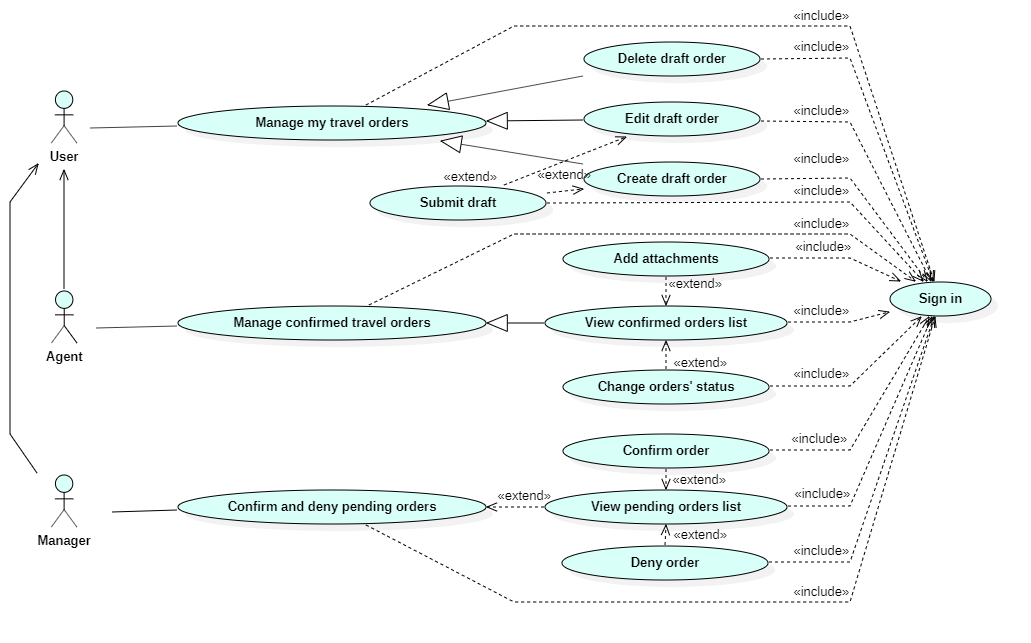
\includegraphics[scale=0.5]{img/sprint3_usecase.png}
        \caption{Sprint 3 use case diagram}
    \end{center}
     \label{fig:my_label}
\end{figure}
         \subsection{Class diagram}
    \begin{figure}[H]
    \begin{center}
        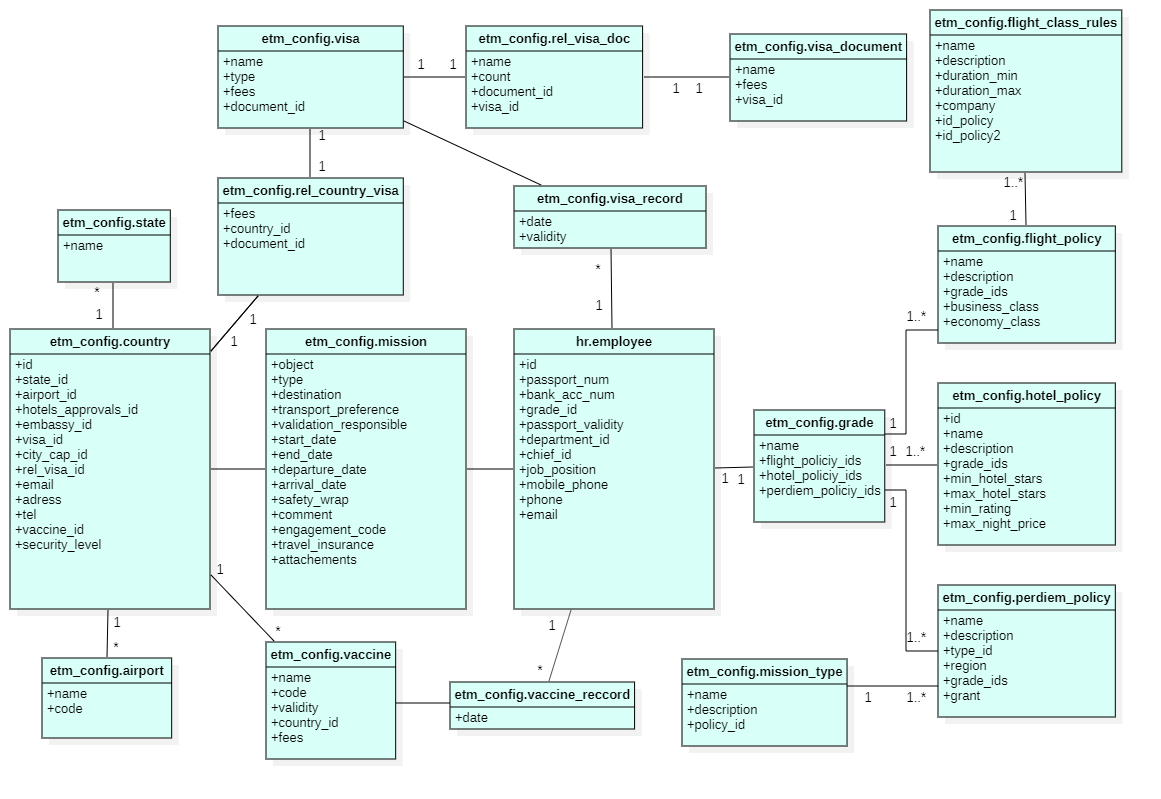
\includegraphics[scale=0.450]{img/sprint3_class.png}
        \caption{Sprint 3 class diagram}
    \end{center}
     \label{fig:my_label}
\end{figure}

In what follows, we will proceed to go in detail on some use cases\\
\subsection*{Use case «Manage my travel orders»}
\begin{figure}[H]
    \begin{center}
        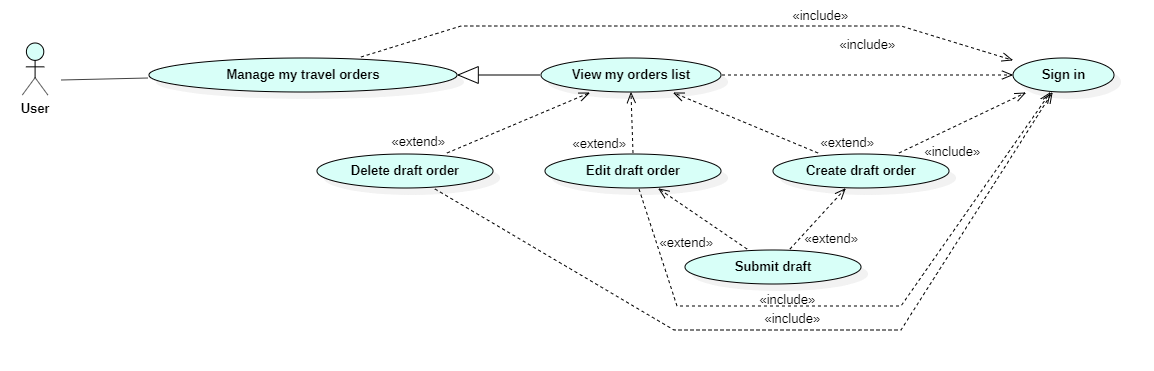
\includegraphics[scale=0.44]{img/sprint3_user_manage_usecase.png}
        \caption{«Manage my travel orders» detailed use case diagram}
    \end{center}
        \label{fig:my_label}
\end{figure} 
The User has the right to create new travel orders at any given time.\\
The User can only edit or delete travel orders that are currently in the "draft" phase.\\
The User can submit a draft order for his superiors to review and process. This order is no longer a draft and is now "pending confirmation"

\begin{center}
\begin{longtable}{|p{4,25cm}|p{9,25cm}|}
\caption{«Create draft order» detailed textual description}
\hline
\textbf{Use Case}&Create draft order
\\\hline
\textbf{Actors}&User
\hline
\textbf{Pre-condition}&User signed in and viewing his orders list
\hline
\textbf{Post-condition}&New draft travel order created
\hline
\textbf{Basic path}&
        \begin{enumerate}
         \item The User clicks on the button "New"
         \item The system displays a a empty form
         \item The User fills the form
         \item The User clicks on the button "Save"
         \item The System processes the input
         \item The System creates a new draft order
         \item The User is sent back to the orders list
     \end{enumerate}\\
\hline
\textbf{Alternative path}&
\begin{itemize}
\item 4.Duplicate or missing Data (The Administrator is sent back to step 2)
\item 2.User clicks on the button "Cancel"(System skips to step 7)
\end{itemize}\\
\hline
\end{longtable}
\end{center}



\subsection*{Use case «Manage confirmed travel orders»}
\begin{figure}[H]
    \begin{center}
        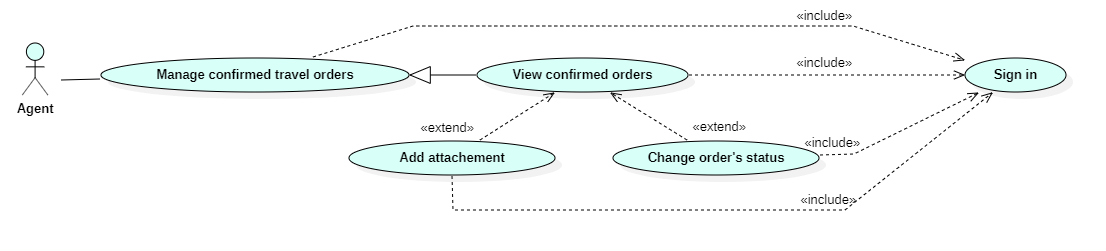
\includegraphics[scale=0.44]{img/sprint3_manage_confirmed_usecase.png}
        \caption{«Manage confirmed travel orders» detailed use case diagram}
    \end{center}
        \label{fig:my_label}
\end{figure} 

The Agent can only process travel orders that the Managers approved.\\
The process is split into 2 main parts :\\
\begin{itemize}
\item Adding attachments (reservations, visa documents, insurance ...)
\item Changing status (ToDo, in progress, Done)
\end{itemize}
\subsubsection*{«Add attachement» sequance diagram}
\begin{figure}[H]
    \begin{center}
        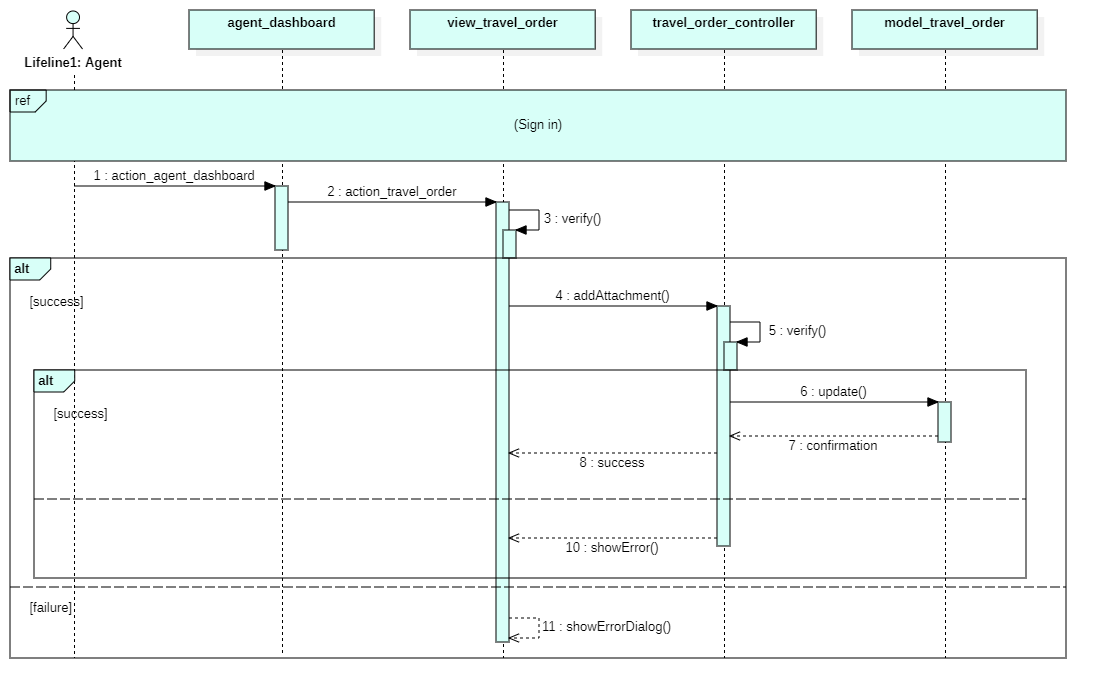
\includegraphics[scale=0.40]{img/sprint3_attach_sequ.png}
        \caption{«Manage confirmed travel orders» detailed use case diagram}
    \end{center}
        \label{fig:my_label}
\end{figure} 

\subsubsection*{Change status textual description}

\begin{center}
\begin{longtable}{|p{4,25cm}|p{9,25cm}|}
\caption{«Create draft order» detailed textual description}
\hline
\textbf{Use Case}&Change order status
\\\hline
\textbf{Actors}&Agent
\hline
\textbf{Pre-condition}&Agent signed in and viewing his dashboard
\hline
\textbf{Post-condition}&order status changed
\hline
\textbf{Basic path}&
        \begin{enumerate}
         \item The Agent drags the travel order card
         \item The Agent drops the card on one of the 3 zones
         \item The System changes the travel order status
     \end{enumerate}\\
\hline
\textbf{Alternative path}&
\begin{itemize}
\item 2.Agent drops the card outside the allocated space (back to step 1)
\item 2.Agent drops a unfinished order card on the "Done" section (back to step1)
\end{itemize}\\
\hline
\end{longtable}
\end{center}




\section{Implementation}
This section presents some user interfaces of the module with screenshots to further clarify our work. The figures below present these interfaces, starting with the first figure which shows the travel order draft. This view is the employee's interface.\\
All employee information is automatically generated and is not editable.\\
All policies are automatically generated (depending on the employee grade and destinations) and are not editable.\\
All Visas and Vaccines are automatically generated (depending on the destinations) and the employee can only change if he have them already or needs to obtain them by checking the checkbox.\\
The Employee can submit this draft by clicking the button above.

\begin{figure}[H]
    \centering
    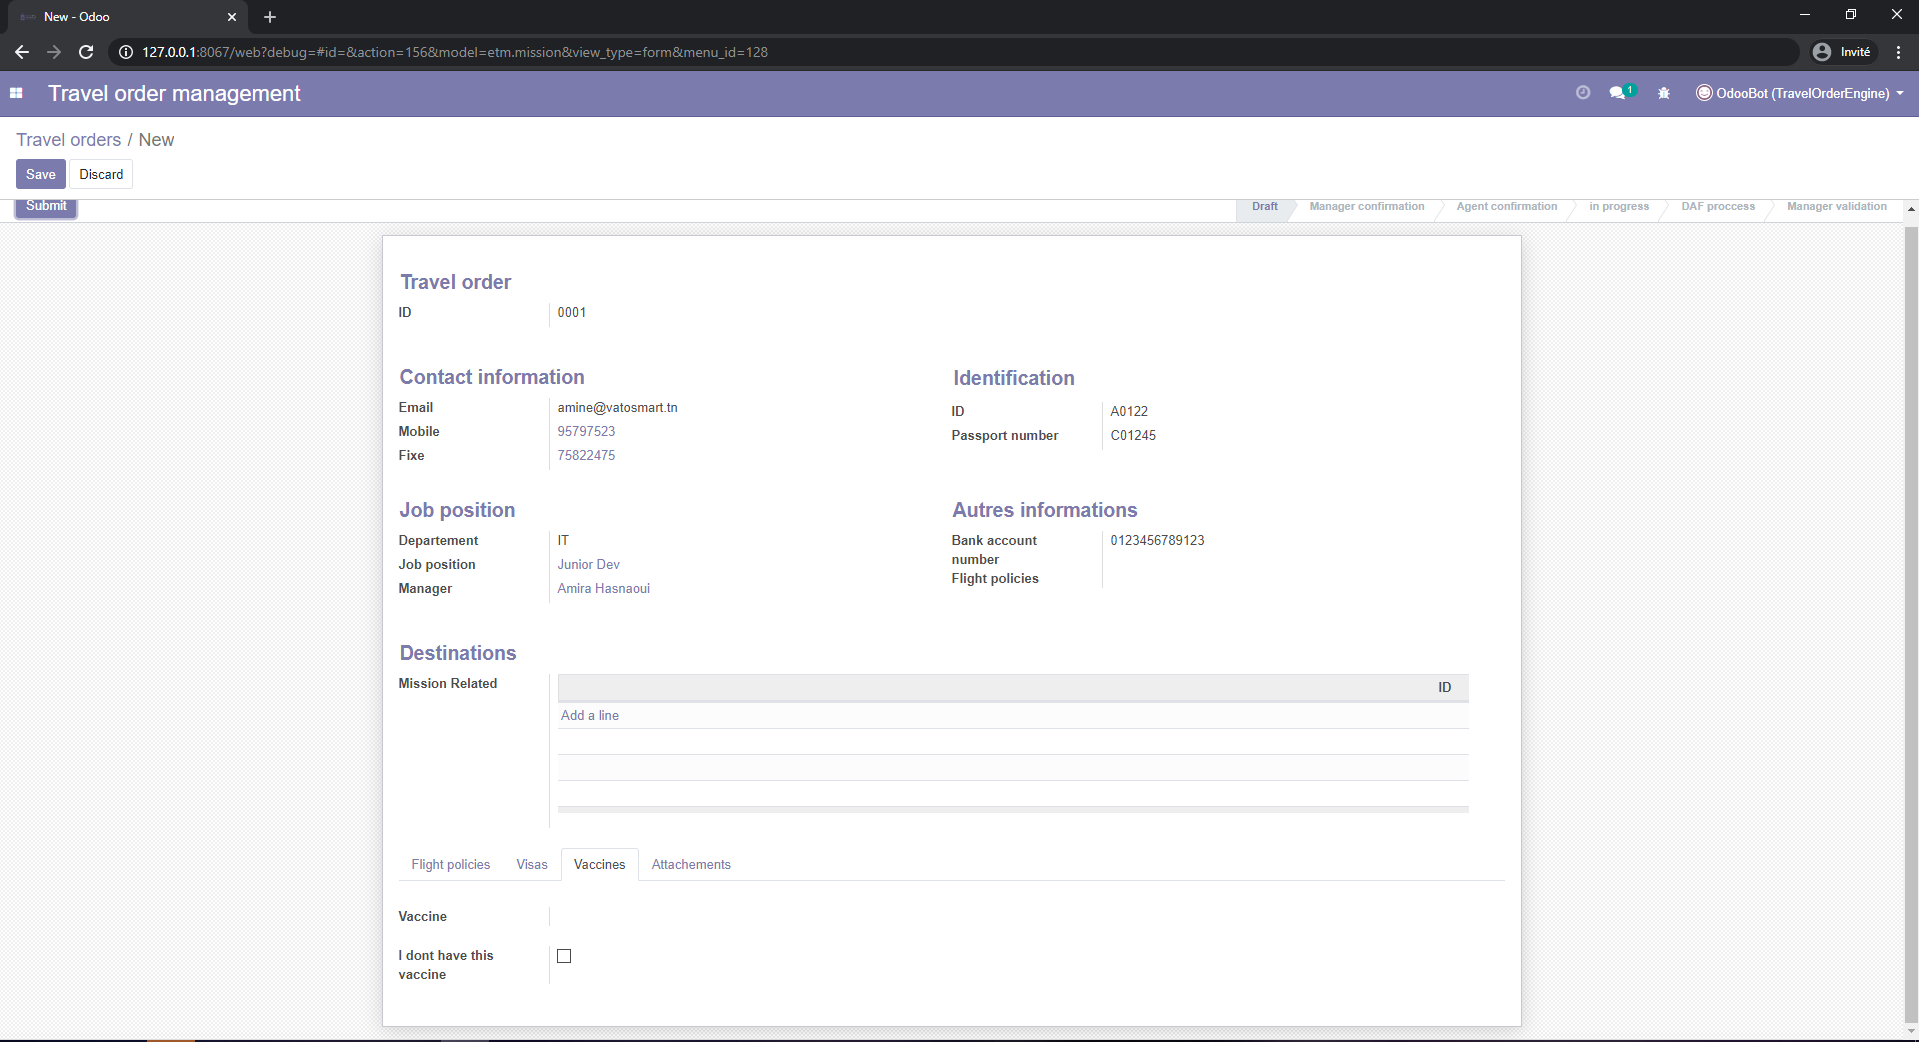
\includegraphics[scale=0.33]{img/c_mission_draft.png}
    \caption{travel order draft view}
    \label{fig:my_label}
\end{figure}

Clicking on the "Add a line" on the destinations list will open a pop-up window that contains a form with all needed information , This figure shows that form view.\\
Policies, Visas, Vaccines are not editable and are automatically generated based on the employee information and the destination country.
\begin{figure}[H]
    \centering
    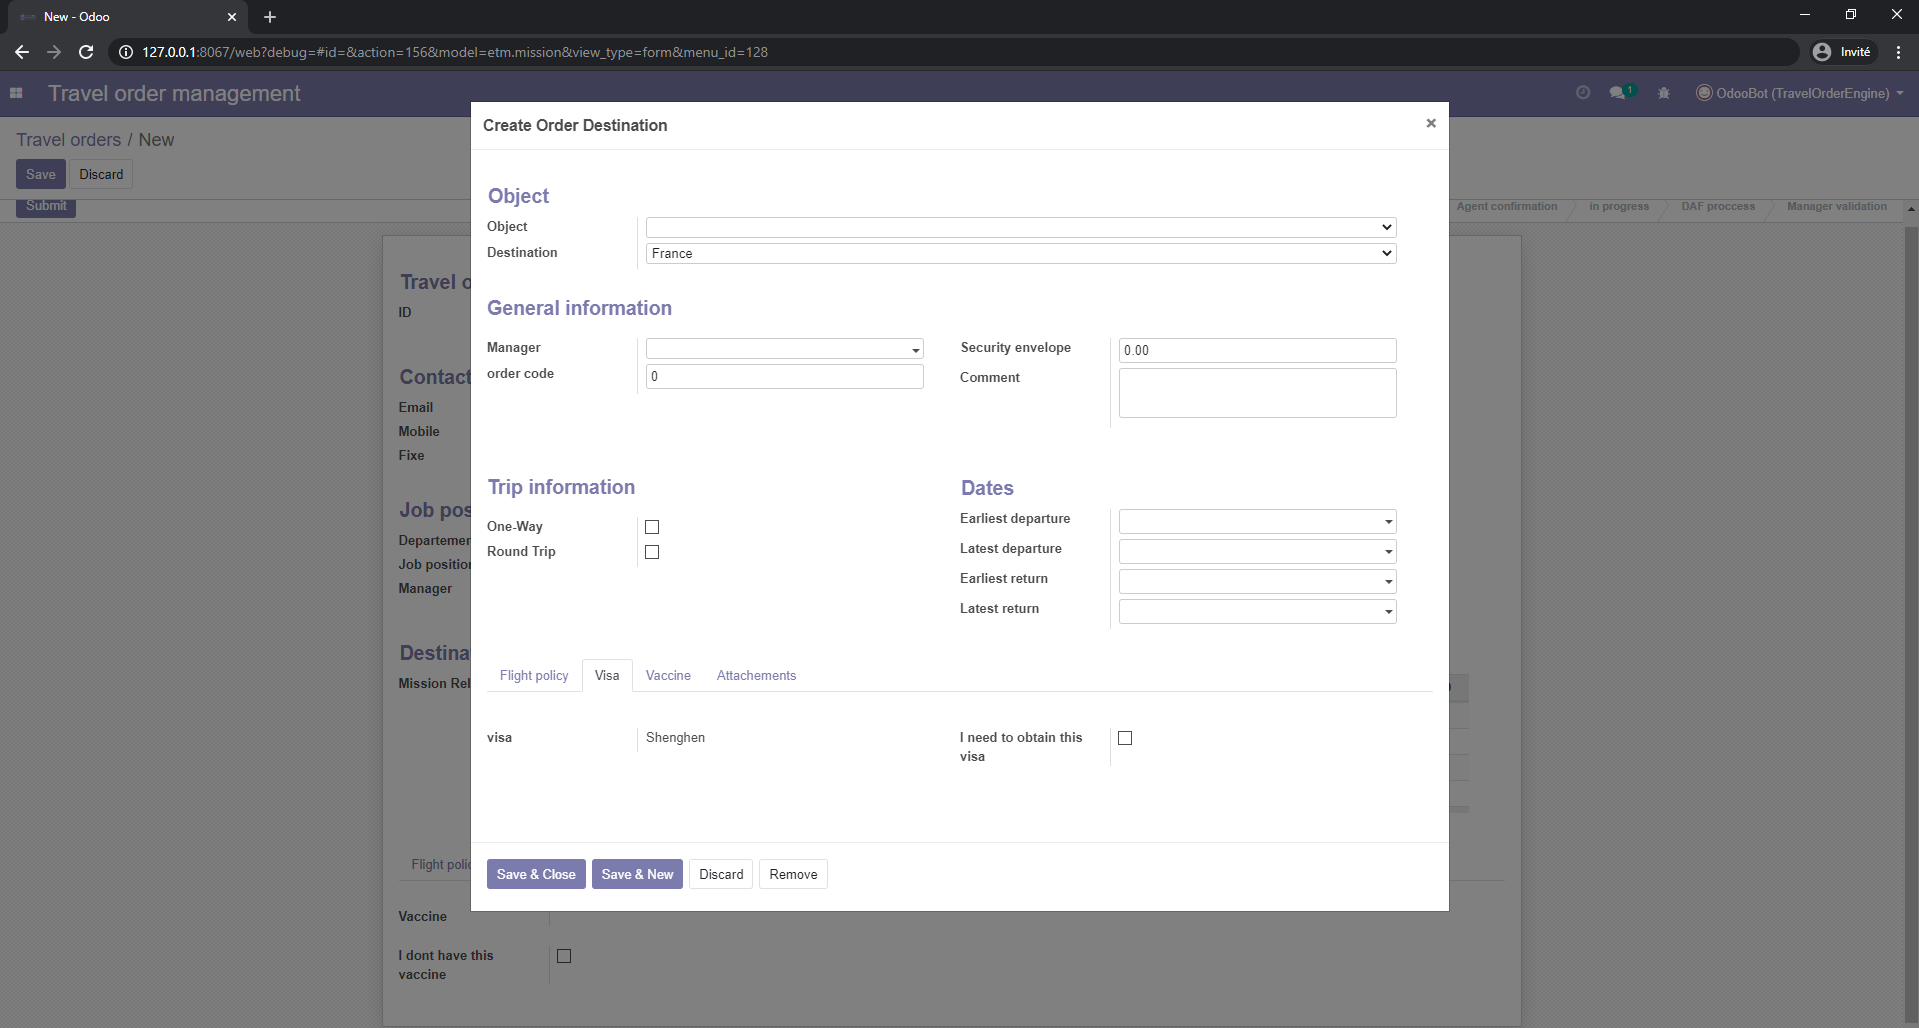
\includegraphics[scale=0.33]{img/c_destination_form.png}
    \caption{travel order destination form}
    \label{fig:my_label}
\end{figure}
The initial manager confirmation, the agent confirmation and the final manager validation are all basically the same static order view but with different workflow state and action buttons. during these phases the actor can only confirm or deny the order. In this figure we will show the manager confirmation
\begin{figure}[H]
    \centering
    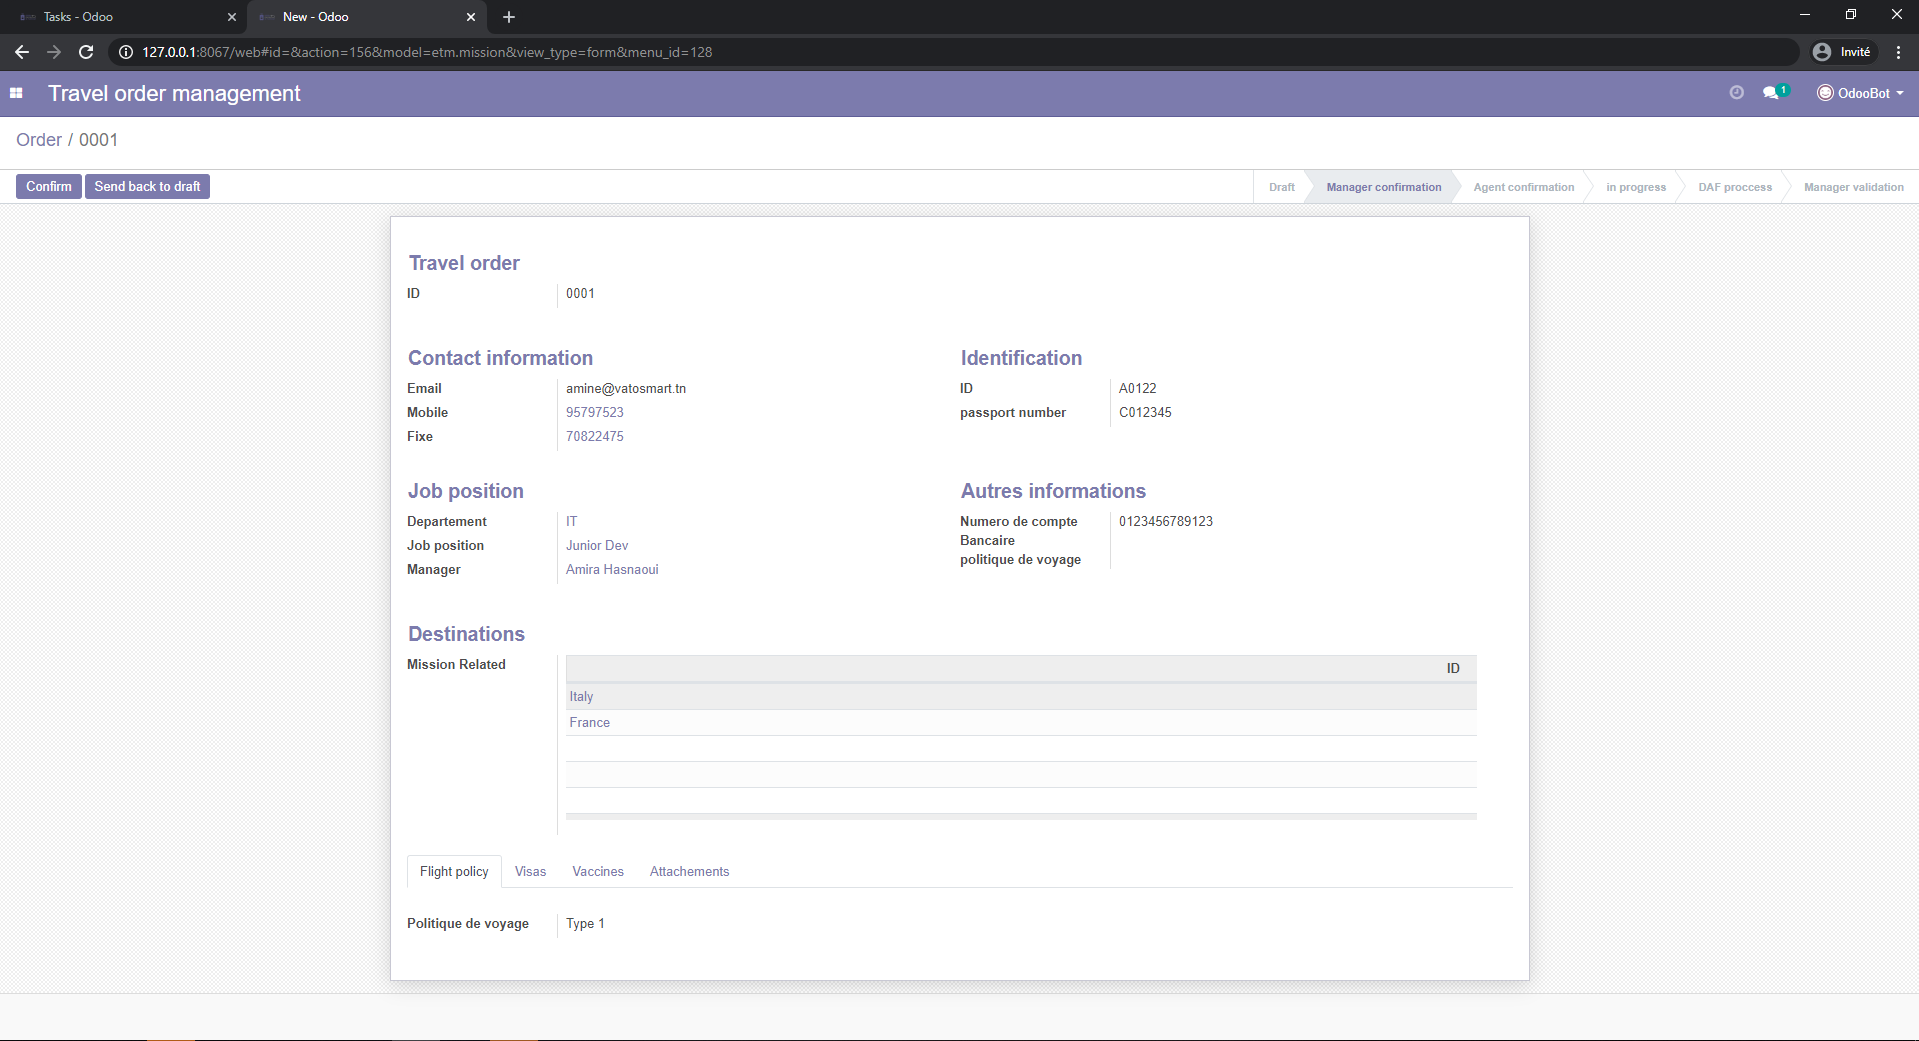
\includegraphics[scale=0.33]{img/c_manager_confirmation.png}
    \caption{Travel order confirmation view}
    \label{fig:my_label}
\end{figure}
In this last figure we will the agent dashboard , where agents can see all approved travel orders and change their status by drag-and-droping the order cards into the "in progress" and "Done" sections.

\begin{figure}[H]
    \centering
    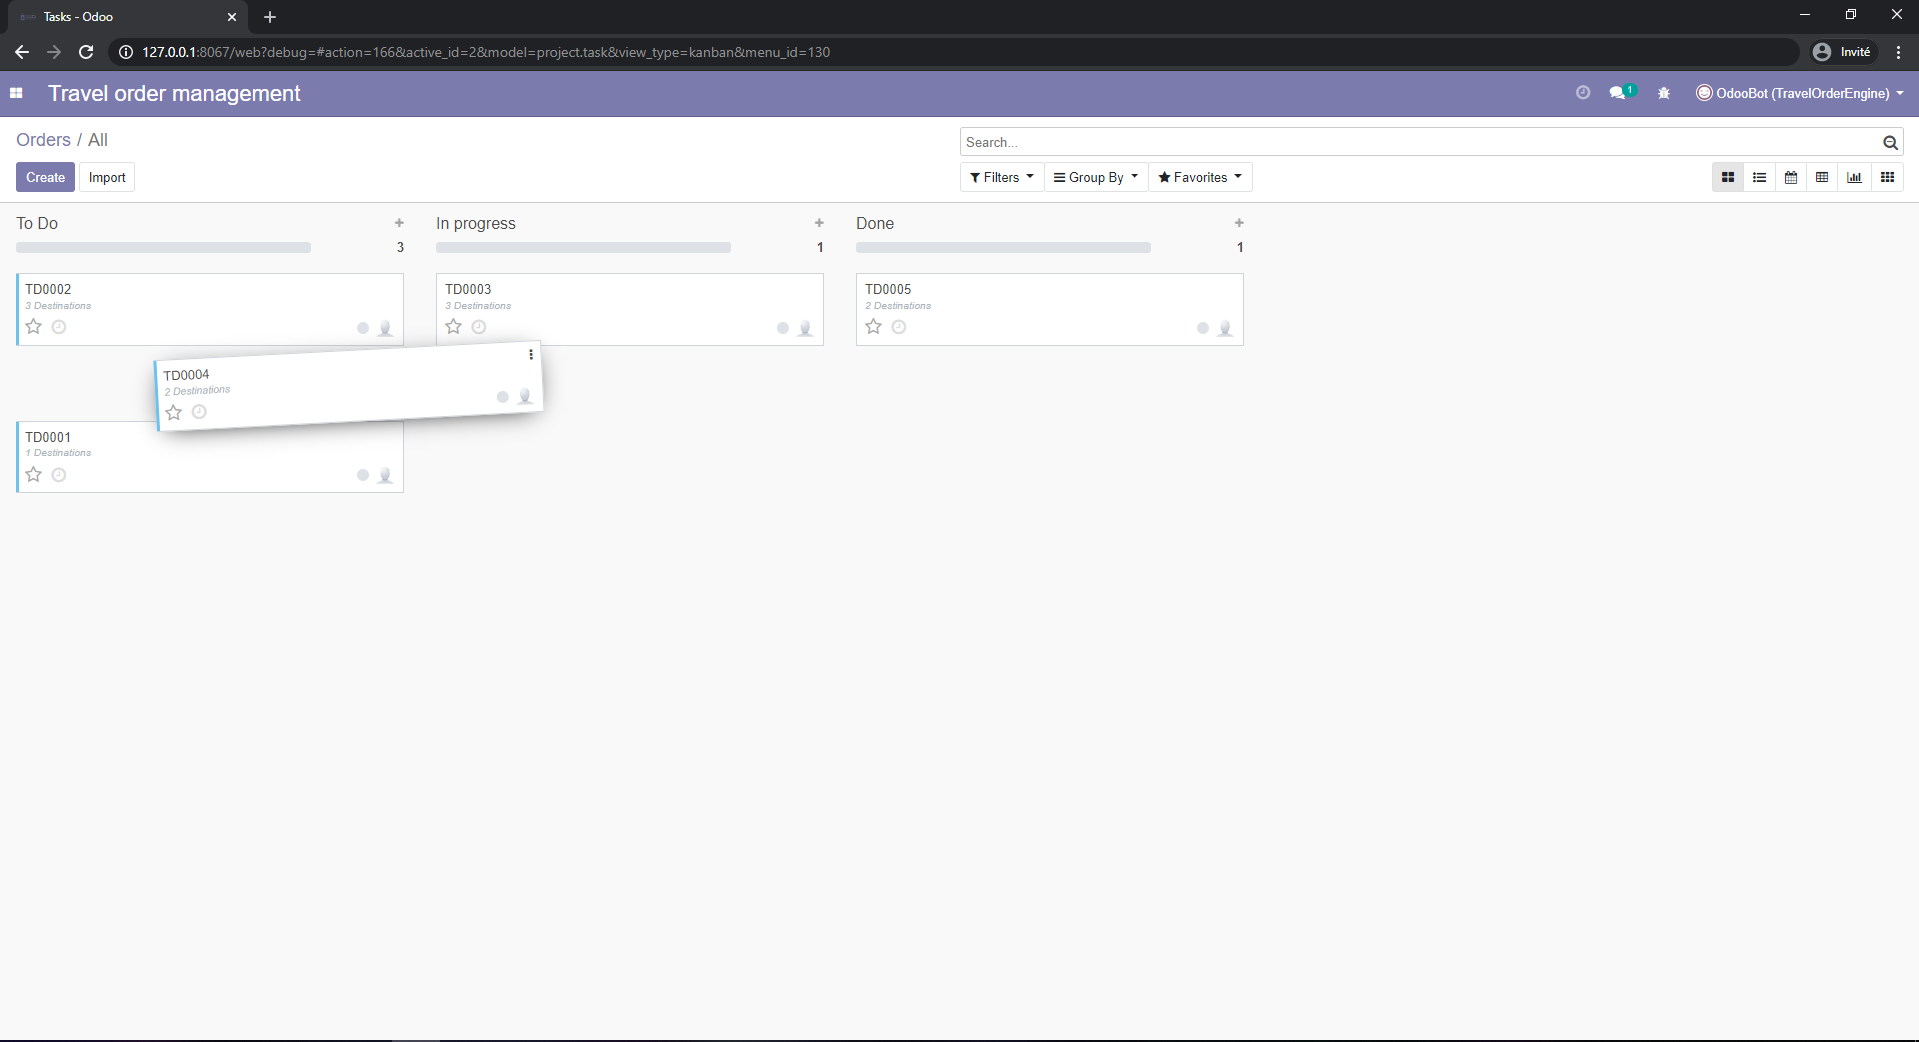
\includegraphics[scale=0.32]{img/c_agent_dash.png}
    \caption{Agent dashboard view}
    \label{fig:my_label}
\end{figure}






\section*{Conclusion}
  This sixth chapter summarized the work done during the third sprint of our project's life cycle, which was the design, development and implementation of a travel order management module. We started with the development of the Backlog sprint,then we started a design phase and we closed this chapter by exposing the interfaces of the developed module.